\chapter{Teoria de jocs}

En aquest capítol, ens centrarem en els jocs de dos jugadors sense
elements aleatoris. El nostre objectiu és trobar una estratègia que
per guanyar el joc independentment del que faci l'oponent, si aquesta
estratègia existeix.

Resulta que hi ha una estratègia general per a aquests jocs, i podem
analitzar els jocs mitjançant la \key{teoria dels jocs de
  nim}. Primer, analitzarem jocs senzills on els jugadors treuen
palets d'una pila, i després generalitzarem l'estratègia utilitzada en
aquests jocs a altres jocs.

\section{Estats del joc}

Considerem un joc on inicialment hi ha una pila de $n$ palets. Els
jugadors $A$ i $B$ es mouen alternativament i el jugador $A$
comença. En cada moviment, el jugador ha de treure 1, 2 o 3 palets de
la pila, i el jugador que treu l'últim palet guanya la partida.

Per exemple, si $n=10$, el joc pot procedir de la següent manera:
\begin{itemize}[noitemsep]
\item El jugador $A$ treu 2 palets (en queden 8).
\item El jugador $B$ treu 3 palets (en queden 5).
\item El jugador $A$ treu 1 palet (queden 4).
\item El jugador $B$ treu 2 palets (queden 2 palets).
\item El jugador $A$ treu 2 palets i guanya.
\end{itemize}

Aquest joc consta d'estats $0,1,2,\ldots,n$, on el nombre de l'estat
és el nombre de palets que queden.

\subsubsection{Estats guanyadors i perdedors}

\index{estat guanyador} \index{estat perdedor}

Un \key{estat guanyador} és un estat on el jugador guanyarà la partida
si juga de manera òptima, i un \key{estat perdedor} és un estat on el
jugador perdrà la partida si l'oponent juga de manera òptima. Resulta
que podem classificar tots els estats d'un joc de manera que cada
estat sigui un estat guanyador o un estat perdedor.

En el joc anterior, l'estat 0 és clarament un estat perdedor, perquè
el jugador no pot fer cap moviment. Els estats 1, 2 i 3 són estats
guanyadors, perquè podem treure 1, 2 o 3 palets i guanyar la
partida. L'estat 4, al seu torn, és un estat perdedor, perquè
qualsevol moviment condueix a un estat que és un estat guanyador per a
l'oponent.

De manera més general, si hi ha un moviment que condueix de l'estat
actual a un estat perdedor, l'estat actual és un estat guanyador i, en
cas contrari, l'estat actual és un estat perdedor. Amb aquesta
observació, podem classificar tots els estats d'un joc començant pels
estats perdedors on no hi ha moviments possibles.

Els estats $0 \ldots 15$ del joc anterior es poden classificar de la
següent manera ($W$ denota un estat guanyador i $L$ denota un estat
perdedor):
\begin{center}
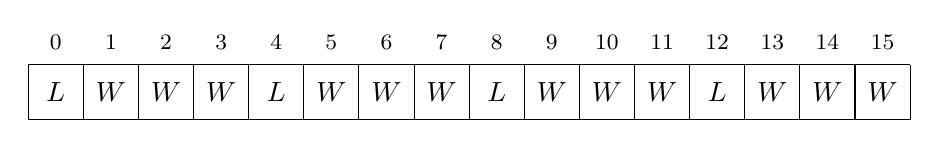
\begin{tikzpicture}[scale=0.7]
\draw (0,0) grid (16,1);

\node at (0.5,0.5) {$L$};
\node at (1.5,0.5) {$W$};
\node at (2.5,0.5) {$W$};
\node at (3.5,0.5) {$W$};
\node at (4.5,0.5) {$L$};
\node at (5.5,0.5) {$W$};
\node at (6.5,0.5) {$W$};
\node at (7.5,0.5) {$W$};
\node at (8.5,0.5) {$L$};
\node at (9.5,0.5) {$W$};
\node at (10.5,0.5) {$W$};
\node at (11.5,0.5) {$W$};
\node at (12.5,0.5) {$L$};
\node at (13.5,0.5) {$W$};
\node at (14.5,0.5) {$W$};
\node at (15.5,0.5) {$W$};

\footnotesize
\node at (0.5,1.4) {$0$};
\node at (1.5,1.4) {$1$};
\node at (2.5,1.4) {$2$};
\node at (3.5,1.4) {$3$};
\node at (4.5,1.4) {$4$};
\node at (5.5,1.4) {$5$};
\node at (6.5,1.4) {$6$};
\node at (7.5,1.4) {$7$};
\node at (8.5,1.4) {$8$};
\node at (9.5,1.4) {$9$};
\node at (10.5,1.4) {$10$};
\node at (11.5,1.4) {$11$};
\node at (12.5,1.4) {$12$};
\node at (13.5,1.4) {$13$};
\node at (14.5,1.4) {$14$};
\node at (15.5,1.4) {$15$};
\end{tikzpicture}
\end{center}


És fàcil analitzar aquest joc: un estat $k$ és un estat perdedor si
$k$ és divisible per 4, i en cas contrari és un estat guanyador. Una
manera òptima de jugar és triar sempre un moviment després del qual el
nombre de palets de la pila és divisible per 4. Finalment, ja no
queden palets i l'oponent ha perdut.

Per descomptat, aquesta estratègia requereix que el nombre de palets
sigui \emph{no} divisible per 4 quan és el nostre moviment. Si és
així, no podem fer res, i el rival guanyarà la partida si juga de
manera òptima.

\subsubsection{Graf d'estats}

Considerem ara un altre joc de palets, on en cada estat $k$, es permet
eliminar qualsevol nombre $x$ de palets de manera que $x$ sigui més
petit que $k$ i divideixi $k$. Per exemple, a l'estat 8 podem treure
1, 2 o 4 palets, però a l'estat 7 l'únic moviment permès és treure 1
palet.

La imatge següent mostra els estats $1 \ldots 9$ del joc com a
\key{graf d'estats}, els nodes del qual són els estats i les arestes
són els moviments entre ells:


\begin{center}
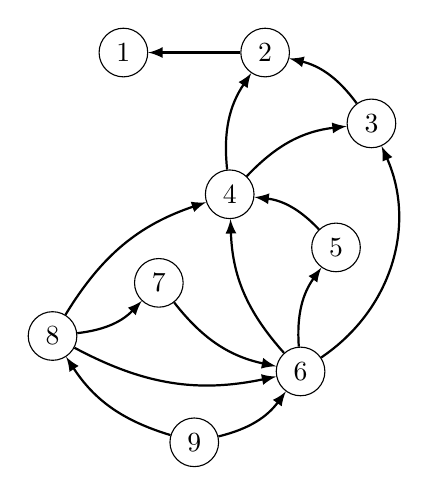
\begin{tikzpicture}[scale=0.9]
\node[draw, circle] (1) at (0,0) {$1$};
\node[draw, circle] (2) at (2,0) {$2$};
\node[draw, circle] (3) at (3.5,-1) {$3$};
\node[draw, circle] (4) at (1.5,-2) {$4$};
\node[draw, circle] (5) at (3,-2.75) {$5$};
\node[draw, circle] (6) at (2.5,-4.5) {$6$};
\node[draw, circle] (7) at (0.5,-3.25) {$7$};
\node[draw, circle] (8) at (-1,-4) {$8$};
\node[draw, circle] (9) at (1,-5.5) {$9$};

\path[draw,thick,->,>=latex] (2) -- (1);
\path[draw,thick,->,>=latex] (3) edge [bend right=20] (2);
\path[draw,thick,->,>=latex] (4) edge [bend left=20] (2);
\path[draw,thick,->,>=latex] (4) edge [bend left=20] (3);
\path[draw,thick,->,>=latex] (5) edge [bend right=20] (4);
\path[draw,thick,->,>=latex] (6) edge [bend left=20] (5);
\path[draw,thick,->,>=latex] (6) edge [bend left=20] (4);
\path[draw,thick,->,>=latex] (6) edge [bend right=40] (3);
\path[draw,thick,->,>=latex] (7) edge [bend right=20] (6);
\path[draw,thick,->,>=latex] (8) edge [bend right=20] (7);
\path[draw,thick,->,>=latex] (8) edge [bend right=20] (6);
\path[draw,thick,->,>=latex] (8) edge [bend left=20] (4);
\path[draw,thick,->,>=latex] (9) edge [bend left=20] (8);
\path[draw,thick,->,>=latex] (9) edge [bend right=20] (6);
\end{tikzpicture}
\end{center}


L'estat final d'aquest joc és sempre l'estat 1, que és un estat
perdedor, perquè no hi ha moviments vàlids. La classificació dels
estats $1 \ldots 9$ és la següent:


\begin{center}
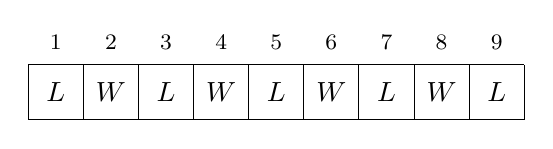
\begin{tikzpicture}[scale=0.7]
\draw (1,0) grid (10,1);

\node at (1.5,0.5) {$L$};
\node at (2.5,0.5) {$W$};
\node at (3.5,0.5) {$L$};
\node at (4.5,0.5) {$W$};
\node at (5.5,0.5) {$L$};
\node at (6.5,0.5) {$W$};
\node at (7.5,0.5) {$L$};
\node at (8.5,0.5) {$W$};
\node at (9.5,0.5) {$L$};

\footnotesize
\node at (1.5,1.4) {$1$};
\node at (2.5,1.4) {$2$};
\node at (3.5,1.4) {$3$};
\node at (4.5,1.4) {$4$};
\node at (5.5,1.4) {$5$};
\node at (6.5,1.4) {$6$};
\node at (7.5,1.4) {$7$};
\node at (8.5,1.4) {$8$};
\node at (9.5,1.4) {$9$};
\end{tikzpicture}
\end{center}


Sorprenentment, en aquest joc, tots els estats parells són estats
guanyadors i tots els estats senars són estats perdedors.

\section{Joc de nim}

\index{joc de nim}

El \key{joc de nim} és un joc senzill que té un paper important en la
teoria de jocs, perquè molts altres jocs es poden jugar amb la mateixa
estratègia. Primer ens centrem en nim, i després generalitzem
l'estratègia a altres jocs.

En el nim hi ha $n$ piles, i cada pila conté un cert nombre de
palets. Els jugadors prenen torns per a triar una pila no buida i
treure qualsevol nombre de palets de la pila. El guanyador és el
jugador que treu l'últim palet.

Els estats a nim tenen la forma $[x_1,x_2,\ldots,x_n]$, on $x_k$
denota el nombre de palets a la pila $k$. Per exemple, $[10,12,5]$ és
un joc on hi ha tres pilas amb 10, 12 i 5 palets. L'estat
$[0,0,\ldots,0]$ és un estat perdedor, perquè no és possible eliminar
cap palet, i és l'únic estat final.

\subsubsection{Anàlisi} \index{suma de nim}

Resulta que podem classificar fàcilment qualsevol estat del joc de nim
calculant la seva \key{suma de nim} $s = x_1 \oplus x_2 \oplus \cdots
\oplus x_n$, on $\oplus$ és l'operació xor\footnote{L'estratègia
òptima per al joc de nim va ser publicada el 1901 per CL Bouton
\cite{bou01}.}. Els estats la suma de nim quals és 0 són estats
perdedors i tots els altres estats són estats guanyadors. Per exemple,
la suma de nim de $[10,12,5]$ és $10 \oplus 12 \oplus 5 = 3$, de
manera que l'estat és un estat guanyador.

Però, com es relaciona la suma de nim amb el joc nim? Podem
explicar-ho mirant com canvia la suma de nim quan canviem l'estat del joc.

\textit{Estats perdedors:} L'estat final $[0,0,\ldots,0]$ és un estat
perdedor, i la seva suma de nim és 0, com s'esperava. En els altres estats
perdedors, qualsevol moviment condueix a un estat guanyador, perquè
quan un sol valor $x_k$ canvia, la suma de nim també canvia, de manera
que la suma de nim és diferent de 0 després del moviment.

\textit{Estats guanyadors:} Ens podem moure a un estat perdedor si
existeix una pila $k$ per a la qual $x_k \oplus s < x_k$. En aquest
cas, podem treure palets de la pila $k$ fins que contingui $x_k \oplus
s$ palets, i per tant sigui un estat perdedor. Sempre hi ha pila
d'aquesta mena, on $x_k$ té un bit 1 a la posició del bit més esquerre
de $s$.

Com a exemple, considereu l'estat $[10,12,5]$. Aquest estat és un
estat guanyador, perquè la seva suma de nim és 3. Per tant, hi ha
d'haver un moviment que condueixi a un estat perdedor. A continuació
descobrirem aquest moviment.

La suma de nim de l'estat és la següent:


\begin{center}
\begin{tabular}{r|r}
10 & \texttt{1010} \\
12 & \texttt{1100} \\
5 & \texttt{0101} \\
\hline
3 & \texttt{0011} \\
\end{tabular}
\end{center}


En aquest cas, la pila amb 10 palets és l'única pila que té un bit 1 a
la posició del bit més esquerre de la suma de nim:


\begin{center}
\begin{tabular}{r|r}
10 & \texttt{10\underline{1}0} \\
12 & \texttt{1100} \\
5 & \texttt{0101} \\
\hline
3 & \texttt{00\underline{1}1} \\
\end{tabular}
\end{center}


La nova mida de la pila ha de ser de $10 \oplus 3 = 9$, de manera que
només treurem un pal. Després d'això, l'estat resultant és $[9,12,5]$,
que és un estat perdedor:


\begin{center}
\begin{tabular}{r|r}
9 & \texttt{1001} \\
12 & \texttt{1100} \\
5 & \texttt{0101} \\
\hline
0 & \texttt{0000} \\
\end{tabular}
\end{center}


\subsubsection{Joc de Misère}

\index{joc de misère}

En un \key{joc de misère}, l'objectiu del joc és oposat, de manera que
el jugador que treu l'últim pal perd la partida. Resulta que el joc de
misère es pot jugar de manera òptima gairebé com el joc de nim estàndard.

La idea és jugar primer al joc de misère com si fos el joc estàndard,
però canviar l'estratègia al final del joc. La nova estratègia
s'introdueix en la situació on cada pila conté com a màxim un pal
després del següent moviment.

Al joc estàndard, hauríem de triar un moviment que ens deixes amb un
nombre parell de piles. Però en el joc de misère triem un moviment
que ens deixi un nombre senar de piles amb un palet.

Aquesta estratègia funciona perquè en el joc sempre apareix un estat
on es possible canviar l'estratègia, i aquest estat és un estat
guanyador, perquè conté exactament una sola pila amb més d'un palet,
de manera que la suma de nim no és 0.

\section{Teorema de Sprague–Grundy}

\index{Teorema de Sprague–Grundy}

El \key{Teorema de Sprague–Grundy}\footnote{El teorema va ser
descobert independentment per R. Sprague \cite{spr35} i PM Grundy
\cite{gru39}.} generalitza l'estratègia utilitzada al joc de nim a
tots els jocs que compleixen els requisits següents:


\begin{itemize}[noitemsep]
\item Dos jugadors prenen torns.
\item El joc consta d'estats. Els moviments que es poden
fer des d'un estat no depenen de quin jugador té el torn.
\item El joc acaba quan un jugador no pot fer un moviment.
\item Es garanteix que el joc acaba tard o d'hora.
\item Els jugadors tenen informació completa sobre
els estats i els moviments, i no hi ha aleatorietat.
\end{itemize}

La idea és calcular per a cada estat del joc un nombre de Grundy que
correspongui al nombre de palets en una pila de nim. Quan coneixem els
nombres de Grundy de tots els estats, podem jugar el joc com si fos
el joc de nim.

\subsubsection{Nombres de Grundy}

\index{Nombres de Grundy} \index{funció mex}

El \key{nombre de Grundy} d'un estat del joc és
\[\textrm{mex}(\{g_1,g_2,\ldots,g_n\}),\]
on $g_1,g_2,\ldots,g_n$ són els nombres de Grundy dels estats als
quals ens podem moure, i la funció mex dóna el nombre no negatiu més
petit que no pertany al conjunt. Per exemple,
$\textrm{mex}(\{0,1,3\})=2$. Si no hi ha moviments possibles en un
estat, el seu nombre de Grundy és $\textrm{mex}(\emptyset)=0$.

Per exemple, en el graf d'estats
\begin{center}
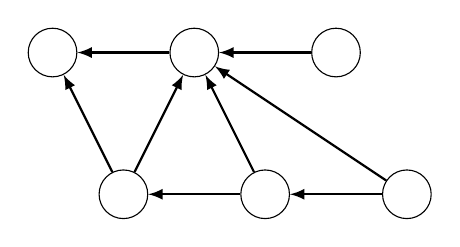
\begin{tikzpicture}[scale=0.9]
\node[draw, circle] (1) at (0,0) {\phantom{0}};
\node[draw, circle] (2) at (2,0) {\phantom{0}};
\node[draw, circle] (3) at (4,0) {\phantom{0}};
\node[draw, circle] (4) at (1,-2) {\phantom{0}};
\node[draw, circle] (5) at (3,-2) {\phantom{0}};
\node[draw, circle] (6) at (5,-2) {\phantom{0}};

\path[draw,thick,->,>=latex] (2) -- (1);
\path[draw,thick,->,>=latex] (3) -- (2);
\path[draw,thick,->,>=latex] (5) -- (4);
\path[draw,thick,->,>=latex] (6) -- (5);
\path[draw,thick,->,>=latex] (4) -- (1);
\path[draw,thick,->,>=latex] (4) -- (2);
\path[draw,thick,->,>=latex] (5) -- (2);
\path[draw,thick,->,>=latex] (6) -- (2);
\end{tikzpicture}
\end{center}
els nombres de Grundy són els següents:
\begin{center}
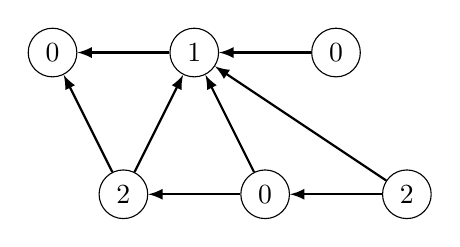
\begin{tikzpicture}[scale=0.9]
\node[draw, circle] (1) at (0,0) {0};
\node[draw, circle] (2) at (2,0) {1};
\node[draw, circle] (3) at (4,0) {0};
\node[draw, circle] (4) at (1,-2) {2};
\node[draw, circle] (5) at (3,-2) {0};
\node[draw, circle] (6) at (5,-2) {2};

\path[draw,thick,->,>=latex] (2) -- (1);
\path[draw,thick,->,>=latex] (3) -- (2);
\path[draw,thick,->,>=latex] (5) -- (4);
\path[draw,thick,->,>=latex] (6) -- (5);
\path[draw,thick,->,>=latex] (4) -- (1);
\path[draw,thick,->,>=latex] (4) -- (2);
\path[draw,thick,->,>=latex] (5) -- (2);
\path[draw,thick,->,>=latex] (6) -- (2);
\end{tikzpicture}
\end{center}
El nombre de Grundy d'un estat perdedor és 0 i el nombre Grundy d'un
estat guanyador és un nombre positiu.

El nombre de Grundy d'un estat s'assembla al nombre de palets en una
pila del joc de nim\footnote{(N. del T.) Excepte que, a diferència del
joc de nim, ara serà possible afegir palets a la pila.}. Si el nombre
de Grundy és 0, només ens podem moure a estats els nombres de Grundy
dels són positius (és a dir, afegir palets), i si el nombre de Grundy
és $x>0$, ens podem moure a estats els nombres de Grundy dels quals
inclouen tots els nombres $0,1,\ldots,x -1$ (és a dir, podem treure
qualsevol nombre de palets).

Com a exemple, considereu un joc on els jugadors mouen una figura en
un laberint. Cada casella del laberint és buida o paret. En cada torn,
el jugador ha de moure la figura uns quants passos cap a l'esquerra o
cap amunt. El guanyador del joc és el jugador que fa l'últim moviment.

La imatge següent mostra un possible estat inicial del joc, on @
indica la figura i * indica una casella on es pot moure.


\begin{center}
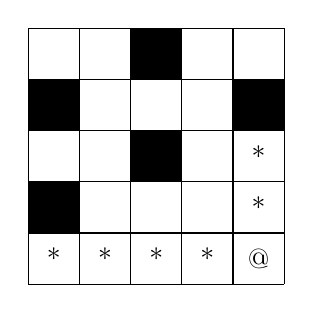
\begin{tikzpicture}[scale=.65]
  \begin{scope}
    \fill [color=black] (0, 1) rectangle (1, 2);
    \fill [color=black] (0, 3) rectangle (1, 4);
    \fill [color=black] (2, 2) rectangle (3, 3);
    \fill [color=black] (2, 4) rectangle (3, 5);
    \fill [color=black] (4, 3) rectangle (5, 4);

    \draw (0, 0) grid (5, 5);
    
    \node at (4.5,0.5) {@};
    \node at (3.5,0.5) {*};
    \node at (2.5,0.5) {*};
    \node at (1.5,0.5) {*};
    \node at (0.5,0.5) {*};
    \node at (4.5,1.5) {*};
    \node at (4.5,2.5) {*};
    
  \end{scope}
\end{tikzpicture}
\end{center}


Els estats del joc són totes les caselles buides. Al laberint
anterior, els nombres de Grundy són els següents:


\begin{center}
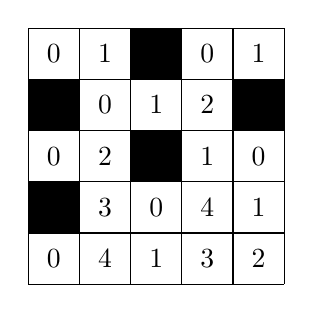
\begin{tikzpicture}[scale=.65]
  \begin{scope}
    \fill [color=black] (0, 1) rectangle (1, 2);
    \fill [color=black] (0, 3) rectangle (1, 4);
    \fill [color=black] (2, 2) rectangle (3, 3);
    \fill [color=black] (2, 4) rectangle (3, 5);
    \fill [color=black] (4, 3) rectangle (5, 4);

    \draw (0, 0) grid (5, 5);
    
    \node at (0.5,4.5) {0};
    \node at (1.5,4.5) {1};
    \node at (2.5,4.5) {};
    \node at (3.5,4.5) {0};
    \node at (4.5,4.5) {1};

    \node at (0.5,3.5) {};
    \node at (1.5,3.5) {0};
    \node at (2.5,3.5) {1};
    \node at (3.5,3.5) {2};
    \node at (4.5,3.5) {};

    \node at (0.5,2.5) {0};
    \node at (1.5,2.5) {2};
    \node at (2.5,2.5) {};
    \node at (3.5,2.5) {1};
    \node at (4.5,2.5) {0};

    \node at (0.5,1.5) {};
    \node at (1.5,1.5) {3};
    \node at (2.5,1.5) {0};
    \node at (3.5,1.5) {4};
    \node at (4.5,1.5) {1};

    \node at (0.5,0.5) {0};
    \node at (1.5,0.5) {4};
    \node at (2.5,0.5) {1};
    \node at (3.5,0.5) {3};
    \node at (4.5,0.5) {2};
  \end{scope}
\end{tikzpicture}
\end{center}


Per exemple, el nombre de Grundy del quadrat inferior dret és 2, de
manera que és un estat guanyador. Podem arribar a un estat perdedor i
guanyar el joc movent-nos quatre passos cap a l'esquerra o dos passos
cap amunt.

Tingueu en compte que és possible moure's a un estat el nombre de
Grundy del qual sigui més gran que el nombre de Grundy de l'estat
actual. Tanmateix, aquesta estratègia mai és útil, ja que l'oponent
sempre pot triar un moviment que cancel·li aquest moviment.

\subsubsection{Subjocs}

A continuació, assumirem que el nostre joc consta de subjocs i, a cada
torn, el jugador escull primer un subjoc i després un moviment al
subjoc. El joc acaba quan no és possible fer cap moviment en cap
subjoc.

En aquest cas, el nombre de Grundy d'un joc és la suma de nim dels
nombres de Grundy dels subjocs. El joc es pot jugar com un joc de nim
calculant tots els nombres de Grundy dels subjocs i després la seva
suma de nim.

Com a exemple, considereu un joc que consta de tres laberints. En
aquest joc, a cada torn, el jugador tria un dels laberints i després
mou la figura al laberint. Suposem que l'estat inicial del joc és el
següent:


\begin{center}
\begin{tabular}{ccc}
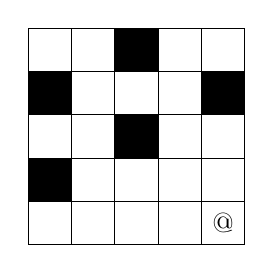
\begin{tikzpicture}[scale=.55]
  \begin{scope}
    \fill [color=black] (0, 1) rectangle (1, 2);
    \fill [color=black] (0, 3) rectangle (1, 4);
    \fill [color=black] (2, 2) rectangle (3, 3);
    \fill [color=black] (2, 4) rectangle (3, 5);
    \fill [color=black] (4, 3) rectangle (5, 4);

    \draw (0, 0) grid (5, 5);

    \node at (4.5,0.5) {@};

    \end{scope}
\end{tikzpicture}
&
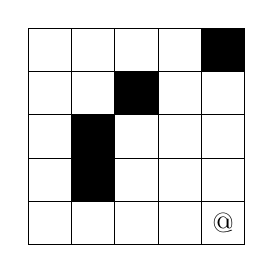
\begin{tikzpicture}[scale=.55]
  \begin{scope}
    \fill [color=black] (1, 1) rectangle (2, 3);
    \fill [color=black] (2, 3) rectangle (3, 4);
    \fill [color=black] (4, 4) rectangle (5, 5);

    \draw (0, 0) grid (5, 5);
    
    \node at (4.5,0.5) {@};

  \end{scope}
\end{tikzpicture}
&
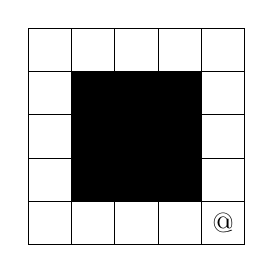
\begin{tikzpicture}[scale=.55]
  \begin{scope}
    \fill [color=black] (1, 1) rectangle (4, 4);

    \draw (0, 0) grid (5, 5);
    
    \node at (4.5,0.5) {@};
  \end{scope}
\end{tikzpicture}
\end{tabular}
\end{center}


Els nombres de Grundy dels laberints són els següents:


\begin{center}
\begin{tabular}{ccc}
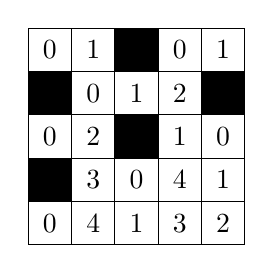
\begin{tikzpicture}[scale=.55]
  \begin{scope}
    \fill [color=black] (0, 1) rectangle (1, 2);
    \fill [color=black] (0, 3) rectangle (1, 4);
    \fill [color=black] (2, 2) rectangle (3, 3);
    \fill [color=black] (2, 4) rectangle (3, 5);
    \fill [color=black] (4, 3) rectangle (5, 4);

    \draw (0, 0) grid (5, 5);

    \node at (0.5,4.5) {0};
    \node at (1.5,4.5) {1};
    \node at (2.5,4.5) {};
    \node at (3.5,4.5) {0};
    \node at (4.5,4.5) {1};

    \node at (0.5,3.5) {};
    \node at (1.5,3.5) {0};
    \node at (2.5,3.5) {1};
    \node at (3.5,3.5) {2};
    \node at (4.5,3.5) {};

    \node at (0.5,2.5) {0};
    \node at (1.5,2.5) {2};
    \node at (2.5,2.5) {};
    \node at (3.5,2.5) {1};
    \node at (4.5,2.5) {0};

    \node at (0.5,1.5) {};
    \node at (1.5,1.5) {3};
    \node at (2.5,1.5) {0};
    \node at (3.5,1.5) {4};
    \node at (4.5,1.5) {1};

    \node at (0.5,0.5) {0};
    \node at (1.5,0.5) {4};
    \node at (2.5,0.5) {1};
    \node at (3.5,0.5) {3};
    \node at (4.5,0.5) {2};
    \end{scope}
\end{tikzpicture}
&
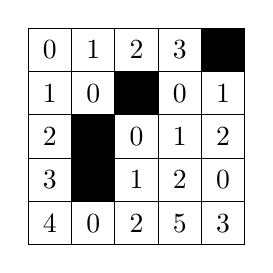
\begin{tikzpicture}[scale=.55]
  \begin{scope}
    \fill [color=black] (1, 1) rectangle (2, 3);
    \fill [color=black] (2, 3) rectangle (3, 4);
    \fill [color=black] (4, 4) rectangle (5, 5);

    \draw (0, 0) grid (5, 5);

    \node at (0.5,4.5) {0};
    \node at (1.5,4.5) {1};
    \node at (2.5,4.5) {2};
    \node at (3.5,4.5) {3};
    \node at (4.5,4.5) {};

    \node at (0.5,3.5) {1};
    \node at (1.5,3.5) {0};
    \node at (2.5,3.5) {};
    \node at (3.5,3.5) {0};
    \node at (4.5,3.5) {1};

    \node at (0.5,2.5) {2};
    \node at (1.5,2.5) {};
    \node at (2.5,2.5) {0};
    \node at (3.5,2.5) {1};
    \node at (4.5,2.5) {2};

    \node at (0.5,1.5) {3};
    \node at (1.5,1.5) {};
    \node at (2.5,1.5) {1};
    \node at (3.5,1.5) {2};
    \node at (4.5,1.5) {0};

    \node at (0.5,0.5) {4};
    \node at (1.5,0.5) {0};
    \node at (2.5,0.5) {2};
    \node at (3.5,0.5) {5};
    \node at (4.5,0.5) {3};
  \end{scope}
\end{tikzpicture}
&
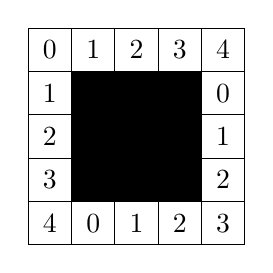
\begin{tikzpicture}[scale=.55]
  \begin{scope}
    \fill [color=black] (1, 1) rectangle (4, 4);

    \draw (0, 0) grid (5, 5);

    \node at (0.5,4.5) {0};
    \node at (1.5,4.5) {1};
    \node at (2.5,4.5) {2};
    \node at (3.5,4.5) {3};
    \node at (4.5,4.5) {4};

    \node at (0.5,3.5) {1};
    \node at (1.5,3.5) {};
    \node at (2.5,3.5) {};
    \node at (3.5,3.5) {};
    \node at (4.5,3.5) {0};

    \node at (0.5,2.5) {2};
    \node at (1.5,2.5) {};
    \node at (2.5,2.5) {};
    \node at (3.5,2.5) {};
    \node at (4.5,2.5) {1};

    \node at (0.5,1.5) {3};
    \node at (1.5,1.5) {};
    \node at (2.5,1.5) {};
    \node at (3.5,1.5) {};
    \node at (4.5,1.5) {2};

    \node at (0.5,0.5) {4};
    \node at (1.5,0.5) {0};
    \node at (2.5,0.5) {1};
    \node at (3.5,0.5) {2};
    \node at (4.5,0.5) {3};
  \end{scope}
\end{tikzpicture}
\end{tabular}
\end{center}


A l'estat inicial, la suma de nim dels nombres de Grundy és $2 \oplus
3 \oplus 3 = 2$, de manera que el primer jugador pot guanyar la
partida. Un moviment òptim és moure dos passos cap amunt en el primer
laberint, que produeix la suma de nim $0 \oplus 3 \oplus 3 = 0$.

\subsubsection{El joc de Grundy}

De vegades, un moviment en un joc divideix el joc en subjocs que són
independents els uns dels altres. En aquest cas, el nombre de Grundy del
joc és


\[\textrm{mex}(\{g_1, g_2, \ldots, g_n \}),\]
on $n$ és el nombre de moviments possibles i
\[g_k = a_{k,1} \oplus a_{k,2} \oplus \ldots \oplus a_{k,m},\]
on el moviment $k$ genera subjocs amb nombres de Grundy $a_{k,1},a_{k,2},\ldots,a_{k,m}$.

\index{El joc de Grundy}

Un exemple d'aquest joc és \key{el joc de Grundy}. Inicialment, hi ha
un sola pila que conté $n$ sticks. En cada torn, el jugador tria una
pila i el divideix en dos piles no buides de manera que les piles
siguin de diferent mida. El jugador que fa l'última jugada guanya la
partida.

Sigui $f(n)$ el nombre Grundy d'una pila que conté $n$ palets. El
nombre de Grundy es pot calcular passant per totes les maneres de dividir
la pila en dos piles. Per exemple, quan $n=8$, les possibilitats són
$1+7$, $2+6$ i $3+5$, de manera que
\[f(8)=\textrm{mex}(\{f(1) \oplus f(7), f(2) \oplus f(6), f(3) \oplus f(5)\}).\]


En aquest joc, el valor de $f(n)$ es basa en els valors de
$f(1),\ldots,f(n-1)$. Els casos base són $f(1)=f(2)=0$, perquè no és
possible dividir les piles d'1 i 2 palets. Els primers nombres de
Grundy són:
\[
\begin{array}{lcl}
f(1) & = & 0 \\
f(2) & = & 0 \\
f(3) & = & 1 \\
f(4) & = & 0 \\
f(5) & = & 2 \\
f(6) & = & 1 \\
f(7) & = & 0 \\
f(8) & = & 2 \\
\end{array}
\]
El nombre de Grundy de $n=8$ és 2, així que és possible guanyar el
joc. El moviment guanyador és crear piles $1+7$, perquè $f(1) \oplus
f(7) = 0$.
